% ------------ %
% tab size = 4 %
% ------------ %


% -----------------------------------------------%
% Content in this presentation is licensed under %
%   a Creative Commons Attribution 3.0 License   %
% -----------------------------------------------%


\documentclass[12pt, hyperref={pdfpagelabels=false}]{beamer} % ------------ %
%                                                                           %
\usepackage[latin1]{inputenc}                                               %
\usepackage[english]{babel}                                                 %
\usepackage[T1]{fontenc}                                                    %
\usepackage{amsmath, amssymb, amsfonts, amsthm}                             %
\usepackage{graphicx}                                                       %
%                                                                           %
\usepackage{ifpdf}                                                          %
\ifpdf                                                                      %
    \usepackage{hyperref}                                                   %
\else                                                                       %
\fi % --------------------------------------------------------------------- %
%
%
%
%
% load the pgf - TikZ package
\usepackage{tikz}
%
% load some TikZ libraries
% - REMARK: do not use blanks or newlines between the libraries
\usetikzlibrary{arrows,decorations.pathmorphing,decorations.footprints,fadings,calc,trees,mindmap,shadows,decorations.text,patterns,positioning,shapes,matrix,fit}
%
% NOTE!! If you want to use the ``intersections' library you have
% to use the latest developement version from www.texample.net
%
%
%
\graphicspath{{../Images/}}

%%%%%%%%%%%%%%%%%%%%%%%%%%%%%%%%%%%%%%%%%%%%%%%%%%%%%%%%%%%%%%%%%

\def\Tikz{Ti\emph{k}Z\ }
%


% in order to remove some warnings
\let\Tiny=\tiny


% as uncovered text should be before being unveiled; options
% -> dynamic	[automatically appear]
% -> invisible	[invisible]
% -> trasparent	[= opacity in %]
\setbeamercovered{invisible}


% theme
%
%\usetheme		[hideothersubsections,left,width=1.8cm]{Hannover}
\usetheme		[]{CambridgeUS}
\usefonttheme	[]{default}
\usecolortheme	[]{default}
\useinnertheme	[]{default}
\useoutertheme	[]{default}


% logo (automatically displaced where the theme requires it)
% the object between curly brackets is a .pdf file
\logo{
\includegraphics[height = 1cm]{logo_dei_small}}


% if you do want the navigation symbols then comment the next line
\setbeamertemplate{navigation symbols}{}


% set background as transparent (otherwise some images could not be seen)
\setbeamercolor{background canvas}{bg=}


% background image
%\setbeamertemplate{background}
%{\centering{\includegraphics[width=\paperwidth,height=\paperheight]{background_image_file}}}


\def\TITLE			{\Tikz Mini Course for Automatic Control People}		% on the first slide
\def\SHORTTITLE		{\Tikz Mini Course}										% on ``testatine''
\def\AUTHOR			{Padova Automatic Control Group}						% on the first slide
\def\SHORTAUTHOR	{Automatic Control Group}								% on ``testatine''
\def\INSTITUTE		{University of Padova - Italy}							% on the first slide
\def\SHORTINSTITUTE	{UniPd}													% on ``testatine''
\def\SUBJECT		{Mini course on \Tikz}
\def\KEYWORDS		{LaTeX, TikZ, figures, Automatic Control People}
\def\CREATOR		{Damiano Varagnolo}
%
\ifpdf \hypersetup
{
	pdftitle		= {\TITLE},
	pdfauthor		= {\AUTHOR},
	pdfsubject		= {\SUBJECT},
	pdfcreator		= {\CREATOR},
	pdfproducer		= {\INSTITUTE},
	pdfkeywords		= {\KEYWORDS},
	%
%	pdfpagemode		= FullScreen,		%
	pdfstartview	= Fit,				% (Fit FitH FitV FitR FitB)
	pdfstartpage	= 1,				%
	pdfnewwindow	= true,				%
	pdfcenterwindow	= true,				%
	pdftoolbar		= false,			% if you want to show Acrobat's toolbar
	pdfmenubar		= false,			% if you want to show Acrobat's menu
	%
	% hyperlinks colors
	colorlinks		= false,			% false: boxed links    true: colored links
	linkbordercolor	= 0.8 0.8 0.8,		% (RGB)
	citebordercolor	= 0.8 0.8 0.8,		% (RGB)
	filebordercolor	= 0.8 0.8 0.8,		% (RGB)
	urlbordercolor	= 0.8 0.8 0.8,		% (RGB)
}
%
\urlstyle{same}							% URL stile
%
\fi
%
\title		[\SHORTTITLE]		{\TITLE}
\author		[\SHORTAUTHOR]		{\AUTHOR}
\date		{}									% keep empty for no dates
\institute	[\SHORTINSTITUTE]	{\INSTITUTE}
%
% if you want the current slide's index
%\author		[\SHORTAUTHOR \\ $\;$ \\ \insertframenumber $\;\!\!$ on \inserttotalframenumber]		{\AUTHOR}


\input{graphical_settings}

\providecommand\thispdfpagelabel[1]{} % add by lian to avoid a bug in
                                % beamer or one need to update beamer
                                % to the newest version
%%%%%%%%%%%%%%%%%%%%%%%%%%%%%%%%%%%%%%%%%%%%%%%%%%%%%%%%%%%%%%%%%
%%%%%%%%%%%%%%%%%%%%%%%%%%%%%%%%%%%%%%%%%%%%%%%%%%%%%%%%%%%%%%%%%
%
\begin{document}
%

\begin{frame}
    %
    \titlepage
    %
    \begin{center}
    \begin{tabular}{ccc}
        %
        \includegraphics[height = 1.3cm]{logo_unipd} &
        %
        $~~~$ &
        %
        
\includegraphics[height = 1.3cm]{logo_dei_big} \\
        %
    \end{tabular}
    \end{center}
    %
    \vspace{0.3cm}
    %
    \begin{center}
        %
        \includegraphics[height = 0.2cm]{creative_commons_license}
        %
        \\
        %
        
\begin{tikzpicture}
            %
            \node[rectangle, font=\tiny, color=gray]
            {Content in this presentation is licensed under a Creative Commons Attribution 3.0 License};
            %
        \end{tikzpicture}
        %
    \end{center}
    %
\end{frame}

\section{Introduction}




\begin{frame}
	%
	\frametitle{Do you like$\ldots$ ?}
	%
	\begin{figure}[!htb]
\begin{center}
\begin{tikzpicture}
[
    xscale  = 1.0,
    yscale  = 1.0,
    transform canvas = {scale = 0.6},
    auto,
    %
    DecisionStyle/.style =
    {
        diamond,
        draw        = blue,
        thick,
        fill        = blue!20,
        text width  = 8em,
        align       = flush center,
        inner sep   = 1pt
    },
    %
    BlockStyle/.style =
    {
        rectangle,
        draw            = blue,
        thick,
        fill            = blue!20,
        text width      = 7.5em,
        align           = center,
        rounded corners,
        minimum height  = 2em
    },
    %
    CloudLineStyle/.style =
    {
        draw,
        ultra thick,
        color   = red,
        -latex,
        shorten >= 2pt,
        dotted
    },
    %
    BlockLineStyle/.style =
    {
        draw,
        ultra thick,
        color   = blue,
        -latex,
        shorten >= 2pt
    },
    %
    CloudStyle/.style =
    {
        draw            = red,
        thick,
        ellipse,
        fill            = red!20,
        minimum height  = 2em
    }
]



\matrix [column sep = 5mm, row sep = 7mm]
{
% row 1
\node [CloudStyle] (expert) {expert};           &
\node [BlockStyle] (init)   {initialize model}; &
\node [CloudStyle] (system) {system};           \\
%
% row 2
                                                            &
\node [BlockStyle] (identify)   {identify candidate model}; &
                                                            \\
%
% row 3
\node [BlockStyle] (update)     {update model};                 &
\node [BlockStyle] (evaluate)   {evaluate candidate models};    &
                                                                \\
%
% row 4
                                                                &
\node [DecisionStyle] (decide)  {is best candidate};            &
                                                                \\
% row 5
                                                                &
\node [BlockStyle] (stop)   {stop};                             &
                                                                \\
}; % end matrix



\draw   [BlockLineStyle]    (init)      -- (identify);
\draw   [BlockLineStyle]    (identify)  -- (evaluate);
\draw   [BlockLineStyle]    (evaluate)  -- (decide);
\draw   [BlockLineStyle]    (update)    |- (identify);
\draw   [BlockLineStyle]    (decide)    -| (update)     node [near start, color = black]    {yes} ;
\draw   [BlockLineStyle]    (decide)    -- (stop)       node [midway, color = black]        {no} ;
\draw   [CloudLineStyle]    (expert)    -- (init);
\draw   [CloudLineStyle]    (system)    -- (init);
\draw   [CloudLineStyle]    (system)    |- (evaluate);



\end{tikzpicture}
\end{center}
\end{figure}



	%
\end{frame}








\begin{frame}
	%
	\frametitle{\Tikz ist kein Zeichenprogramm}
	%
	\begin{center}
	\begin{tikzpicture}
		%
		\node [WarningTextStyle] {why should we use \Tikz for drawings?};
		%
	\end{tikzpicture}
	\end{center}
	%
	\uncover<1->
	{
		\alert{Advantages w.r.t.\ other drawing methods:}
		%
		\begin{itemize}
			\item extremely simple for logically simple drawings
			\item usage of \emph{native code} $\Rightarrow$ portable
			\item text and styles are the standard \LaTeX\ ones
			\item modification of existing drawings can be \alert{orders of magnitudo} more rapid (seconds vs.\ hours)
		\end{itemize}
	}
	%
\end{frame}





\begin{frame}
	%
	\frametitle{\Tikz ist kein Zeichenprogramm}
	%
	\begin{center}
	\begin{tikzpicture}
		%
		\node [WarningTextStyle] {why should we \textbf{\alert{do not}} use \Tikz for drawings?};
		%
	\end{tikzpicture}
	\end{center}
	%
	\uncover<1->
	{
		\alert{Disadvantages w.r.t.\ other drawing methods:}
		%
		\begin{itemize}
			\item quite slow when starting learning
			\item complicated for ``logically complicated'' pictures
			\item production of the first drafts can be \alert{orders of magnitudo} slower (hours vs.\ minutes)
		\end{itemize}
	}
	%
\end{frame}





\begin{frame}
	%
	\frametitle{General advice}
	%
	\uncover<1->
	{
		\begin{center}
		\begin{tikzpicture}
			%
			\node [WarningTextStyle]
			{read the chapter on ``Guidelines on Graphics'' on the \Tikz manual! (1.7)};
			%
		\end{tikzpicture}
		\end{center}
		%
		%
		general guidelines and principles concerning the \alert{creation of graphics for scientific presentations, papers, and books}
	}
	%
\end{frame}






\begin{frame}
	%
	\frametitle{Warning for the \LaTeX\ source code of this guide}
	%
	\begin{center}
	\begin{tikzpicture}
		%
		\node
		[WarningTextStyle]
		{In the \texttt{.tex} files of this presentation you may find someting like ``\texttt{uncover<1->}'': they are BEAMER commands, not \Tikz commands!!};
		%
	\end{tikzpicture}
	\end{center}
	%
	if you want to use this code you should cancel them
	%
\end{frame}





\begin{frame}
	%
	\frametitle{Where to obtain \Tikz}
	%
	\begin{description}
		%
		\item[stable version:]<1-> \texttt{pgf2.0} - official versions available in:
			%
			\vspace{0.3cm}
			%
			\begin{itemize}
				\item<1-> CTAN: \url{http://www.ctan.org/}
				\vspace{0.1cm}
				\item<1-> SourceForge: \url{http://sourceforge.net/projects/pgf/}
			\end{itemize}
		%
		\vspace{1.0cm}
		%
		\item[developement version:]<2-> \url{http://www.texample.net}
		%
	\end{description}
	%
\end{frame}





\begin{frame}
	%
	\frametitle{Where to obtain the developement version}
	%
	\begin{center}
	\begin{tikzpicture}
		%
		\uncover<1->
		{
			\node (nUrl) [sTextBlockStyle] {URL: \url{http://www.texample.net}};
		}
		%
		\uncover<2->
		{
			\node (nFirstSelect) [sTextBlockStyle, below = of nUrl] {select \Tikz};
			\draw [-open triangle 45, thick] (nUrl) to (nFirstSelect);
		}
		%
		\uncover<3->
		{
			\node (nSecondSelect) [sTextBlockStyle, below = of nFirstSelect] {download ``latest build''};
			\draw [-open triangle 45, thick] (nFirstSelect) to (nSecondSelect);
		}
		%
		\uncover<4->
		{
			\node (nInstallation) [sTextBlockStyle, below = of nSecondSelect]
				{install the (TDS-compliant) package};
			\draw [-open triangle 45, thick] (nSecondSelect) to (nInstallation);
		}
		%
		\uncover<5->
		{
			\node [sTextBlockStyle, below = of nSecondSelect, text = red, draw = red]
				{install the (TDS-compliant) package};
			\node (nQuestion) [below of = nInstallation] {don't know how? Google it!};
		}
		%
		%
	\end{tikzpicture}
	\end{center}
	%
\end{frame}




\begin{frame}
	%
	\frametitle{The most important advice:}
	%
	\uncover<2->
	{
		\begin{center}
		\begin{tikzpicture}
		[transform canvas = {scale = 1.5}]
				%
				\pattern
				[
					pattern color	= blue!25,
					pattern			= fivepointed stars,
					path fading	= middle,
				]
				(-5,-2) rectangle (5,2);
				%
				\node[color = red!90!black]
				{\Large{\textbf{\Tikz manual is your friend!}}};
				%
		\end{tikzpicture}
		\end{center}
	}
	%
\end{frame}




\section{Basic concepts}



\begin{frame}
	%
	\frametitle{Environment declaration}
	%
	\begin{itemize}
		%
		\item template file for floating figures: \\
			\begin{center}
				\url{./Sources/template__floating_figure_declaration.tex}
			\end{center}
		%
		\vspace{1cm}
		%
		\item template file for non floating figures: \\
			\begin{center}
				\url{./Sources/template__non_floating_figure_declaration.tex}
			\end{center}
		%
	\end{itemize}
	%
\end{frame}









\begin{frame}
	%
	\frametitle{First main objects: nodes}
	%
	Main properties:
	%
	\begin{itemize}
		\item they are labelled (in order to be referenced)
		\item they can be placed everywhere
		\item you can write \LaTeX\ code inside them
		\item can be \emph{fully} customized
	\end{itemize}
	%
	\vspace{1cm}
	%
	(example file: \url{./Sources/basic_concepts__nodes_examples.tex})
	%
	\begin{figure}[!htb]
\begin{center}
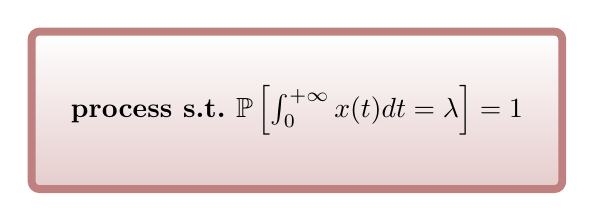
\begin{tikzpicture}
[
	xscale	= 1,	% to scale horizontally everything but the text
	yscale	= 1,	% to scale vertically everything but the text
]

\node
(nProcessNode)							% name of the node
[										% properties of the node:
	shape			= rectangle,		% shape
	rounded corners	= 0.1cm,			% roundness of the corners
	minimum height	= 2cm,				% | minimum size
	minimum width	= 6cm,				% |
	line width		= 0.1cm,			% thickness of the border
	draw			= red!50!black!50,	% colour of the border
	top color		= white,			% | filling colors
	bottom color	= red!50!black!20,	% |
	font			= \bfseries,		% used font
	inner xsep		= 0.5cm,			% minimum distance btw text and borders along x dimension
	inner ysep		= 0.5cm				% minimum distance btw text and borders along y dimension
]
{process s.t.\ $\mathbb{P} \left[ \int_{0}^{+\infty} x(t) dt = \lambda \right] = 1$}; % DON'T FORGET THE SEMICOLON!!

\end{tikzpicture}
\end{center}
\end{figure}

	%
\end{frame}





\begin{frame}
	%
	\frametitle{Second main objects: paths}
	%
	Main properties:
	%
	\begin{itemize}
		\item can be drawn everywhere - connect everything
		\item can have text along them
		\item can be \emph{fully} customized
	\end{itemize}
	%
	\vspace{1cm}
	%
	(example file: \url{./Sources/basic_concepts__paths_examples.tex})
	%
	\begin{figure}[!htb]
\begin{center}
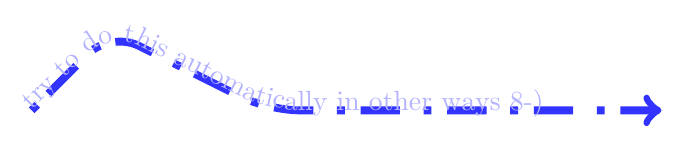
\begin{tikzpicture}
[
	xscale	= 1,	% to scale horizontally everything but the text
	yscale	= 1,	% to scale vertically everything but the text
]

\draw
[
	->,										% kind of line
	rounded corners		= 0.4cm,			% behavior of the corners
	color				= blue!80!white,	%
	line width			= 0.1cm,			%
	dash pattern		= on 0.1cm    off 0.2cm    on 0.5cm    off 0.3cm,
	%
	postaction			=					% after having drawn the line ...
	{										%
		decorate,							% decorate it
		decoration		=					% with which decoration?
		{
			text along path,				% with some text...
			text			= {try to do this automatically in other ways 8-)}, % ...(this text)...
			text color		= blue!30!white	% ...of this color
		}
	}
]
(0cm,0cm) -- (1cm,1cm) -- (3cm,0cm) -- (8cm,0cm); % DON'T FORGET THE SEMICOLON!!

\end{tikzpicture}
\end{center}
\end{figure}

	%
\end{frame}





\begin{frame}
	%
	\frametitle{Well, not all can be done in a single presentation$\ldots$}
	%
	\begin{center}
	\begin{tikzpicture}
		%
		\node [WarningTextStyle]
		{and the coordinates specification??};
		%
	\end{tikzpicture}
	\end{center}
	%
	too time consuming to be fully explained! We'll use only:
	%
	\begin{itemize}
		%
		\item absolute coordinates (like \texttt{at (1.3cm, 2.1cm)})
		%
		\item relative coordinates (like \texttt{above this guy, left of this other})
		%
	\end{itemize}
	%
	\uncover<2->
	{
		\begin{center}
		
\begin{tikzpicture}
			%
			\node [scope fading = east]
			{\large{again: \alert{take a look a the manual$\ldots\ldots\ldots$}}};
			%
		\end{tikzpicture}
		\end{center}
	}
	%
\end{frame}


\section{Nodes}
\label{sec:nodes}




\begin{frame}
	%
	\frametitle{Nodes: how to set the shape}
	%
	(example file: \url{./Sources/nodes__examples_of_shapes.tex} - using \texttt{shapes} library)
	%
	\begin{figure}[!htb]
\begin{center}
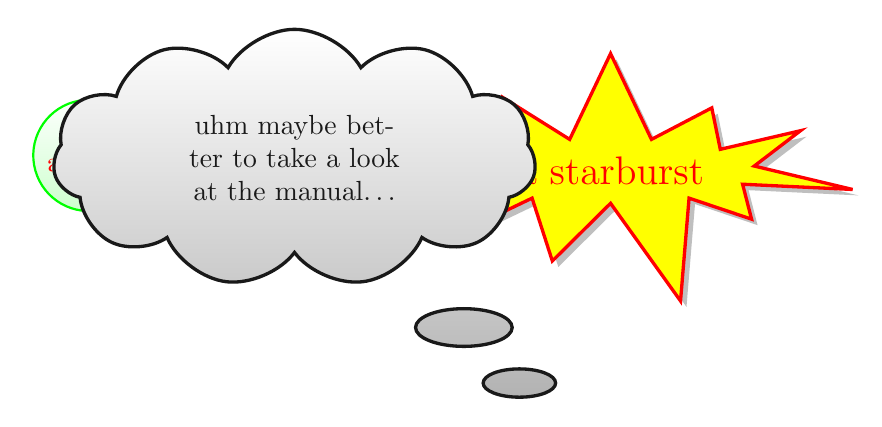
\begin{tikzpicture}
[
	xscale	= 1,						% to scale horizontally everything but the text
	yscale	= 1,						% to scale vertically everything but the text
]

\uncover<1->
{
	\node
	(nCircle)
	[
		shape			= circle,
		top color		= white,			% | filling of the node
		bottom color	= green!20!white,	% |
		text			= red,				% colour of the fonts
		draw			= green,			% colour of the border
		rotate			= 10,				% angle of rotation
		thick,								% thickness of the border
	]
	{a circle};								% note: position not specified!
}

\uncover<2->
{
	\node
	(nStar)
	[
		right = of		  nCircle,			% position
		shape			= star,				% shape
		draw			= blue,				% colour of the border
		top color		= white,			% | filling of the node
		bottom color	= blue!20!white,	% |
		text			= blue,				% colour of the fonts
		rotate			= -10,				% angle of rotation
		thick,								% thickness of the border
	]
	{a star};
}

\uncover<3->
{
	\node
	(nStarburst)
	[
		right = of		  nStar,			% position
		shape			= starburst,		% shape
		starburst points		= 11,		% | shape parameters
		starburst point height	= 1.5cm,	% |
		draw			= red,				% colour of the border
		top color		= yellow,			% | filling of the node
		bottom color	= yellow,			% |
		text			= red,				% colour of the fonts
		font			= \Large,			% shape of the font
		rotate			= 0,				% angle of rotation
		very thick,							% thickness of the border
		drop shadow,
	]
	{a starburst};
}

\uncover<4->
{
	\node
	(nCloudCallout)
	[
		% shape and shape properties
		shape						= cloud callout,
		cloud puffs					= 11,
		aspect						= 2.5,
		cloud puff arc				= 120,
		callout pointer start size	= .25 of callout,
		callout pointer end size	= .15 of callout,
		callout relative pointer	= {(315:2cm)},	% angle - distance
		callout pointer segments	= 2,
		%
		draw			= black!90!white,	% colour of the border
		top color		= white,			% | filling of the node
		bottom color	= black!30!white,	% |
		text			= black!90!white,	% colour of the fonts
		text width		= 4cm,				%
		align			= center,			% text alignment
		very thick,							% thickness of the border
	]
	at (nStar)
	{uhm maybe better to take a look at the manual$\ldots$};
}

\end{tikzpicture}
%
\end{center}
\end{figure}


	%
\end{frame}





\begin{frame}
	%
	\frametitle{Avoid hard coding: styles definitions will make you save LOTS of time}
	%
	\begin{center}
	\begin{tikzpicture}
		%
		\node [WarningTextStyle] {declare the styles in a \\ separate file and input it somewhere};
		%
	\end{tikzpicture}
	\end{center}
	%
	(example file: \url{./Sources/graphical_settings.tex})
	%
\end{frame}




\subsection{Positioning}
\label{ssec:positioning}


\begin{frame}
	%
	\frametitle{Nodes positioning: absolute coordinates}
	%
	we can place the various nodes using absolute coordinates \\
	%
	(example file: \url{./Sources/nodes__absolute_positioning.tex})
	%
	\begin{figure}[!htb]
\begin{center}
\begin{tikzpicture}
[
	xscale	= 1,	% to scale horizontally everything but the text
	yscale	= 1,	% to scale vertically everything but the text
]


\node (nSensorOne)		[SensorNodeStyle]	at	(-0.8, 0.5)	{1};
\node (nSensorTwo)		[SensorNodeStyle]	at	(1.3, 0.9)	{2};
\node (nSensorThree)	[SensorNodeStyle]	at	(0.4, -0.9)	{3};
\node (nBayStation)		[BayStationStyle]	at	(0, 0)		{bs};


\end{tikzpicture}
\end{center}
\end{figure}


	%
\end{frame}




\begin{frame}
	%
	\frametitle{Nodes positioning: relative coordinates}
	%
	place the various nodes using relative coordinates \\
	%
	(example file: \url{./Sources/nodes__relative_positioning.tex})
	%
	\begin{figure}[!htb]
\begin{center}
\begin{tikzpicture}
[
	xscale	= 1,	% to scale horizontally everything but the text
	yscale	= 1,	% to scale vertically everything but the text
]


\node (nSensorOne)		[SensorNodeStyle]							{1};
\node (nSensorTwo)		[SensorNodeStyle, right of = nSensorOne]	{2};
\node (nSensorThree)	[SensorNodeStyle, right of = nSensorTwo]	{3};
\node (nBayStation)		[BayStationStyle, below of = nSensorTwo]	{bs};


\end{tikzpicture}
\end{center}
\end{figure}


	%
\end{frame}





\begin{frame}
	%
	\frametitle{Nodes positioning: matricial positioning}
	%
	place the various nodes inside a matrix \\
	%
	(example file: \url{./Sources/nodes__matricial_positioning.tex} - requires \texttt{matrix} library)
	%
	\begin{figure}[!htb]
\begin{center}
\begin{tikzpicture}
[
	xscale	= 1,	% to scale horizontally everything but the text
	yscale	= 1,	% to scale vertically everything but the text
]



\matrix
(mnMatrixOfNodes)	% this is the name of the ``super node''
[
	matrix of nodes,
	right delimiter	= \rmoustache,
	above delimiter	= \{,
	row sep			= 5mm,
	column sep		= 5mm
]
{
	% first row
	\node (nSensorOne) [SensorNodeStyle] {1}; & % DON'T FORGET SEMICOLONS!!
	&
	&
	\node (nSensorTwo) [SensorNodeStyle] {2}; \\ % DON'T FORGET SEMICOLONS!!
	%
	%
	% second row
	&
	&
	\node (nSensorThree) [SensorNodeStyle] {3}; & % DON'T FORGET SEMICOLONS!!
	\\
	%
	%
	% third row
	&
	\node (nSensorFour) [SensorNodeStyle] {4}; & % DON'T FORGET SEMICOLONS!!
	&
	\node (nBayStation) [BayStationStyle] {bs}; \\ % DON'T FORGET SEMICOLONS!!
};



\end{tikzpicture}
\end{center}
\end{figure}


	%
	(read the manual! This library has \alert{really useful tools}!)
	%
\end{frame}

 




\begin{frame}
	%
	\frametitle{Automatic fit of sets of nodes}
	%
	(example file: \url{./Sources/nodes__fitting_sets_of_nodes.tex} - requires \texttt{fit} library)
	%
	\begin{figure}[!htb]
\begin{center}
\begin{tikzpicture}
[
	xscale = 1.0,
	yscale = 1.0
]



\uncover<1->
{
	\node (nBayStation) [BayStationStyle] at \BayStationPosition {bs};
	\node (nSensorOne)		[SensorNodeStyle] at \SensorOnePosition			{1};
	\node (nSensorTwo)		[SensorNodeStyle] at \SensorTwoPosition			{2};
	\node (nSensorThree)	[SensorNodeStyle] at \SensorThreePosition		{3};
	\node (nSensorFour)		[SensorNodeStyle] at \SensorFourPosition		{4};
	\node (nSensorFive)		[SensorNodeStyle] at \SensorFivePosition		{5};
	\node (nSensorSix)		[SensorNodeStyle] at \SensorSixPosition			{6};
	\node (nSensorSeven)	[SensorNodeStyle] at \SensorSevenPosition		{7};
	\node (nSensorEight)	[SensorNodeStyle] at \SensorEightPosition		{8};
	\node (nSensorNine)		[SensorNodeStyle] at \SensorNinePosition		{9};
	\node (nSensorTen)		[SensorNodeStyle] at \SensorTenPosition			{10};
	\node (nSensorEleven)	[SensorNodeStyle] at \SensorElevenPosition		{11};
	\node (nSensorTwelve)	[SensorNodeStyle] at \SensorTwelvePosition		{12};
	\node (nSensorThirteen)	[SensorNodeStyle] at \SensorThirteenPosition	{13};
	\node (nSensorFourteen)	[SensorNodeStyle] at \SensorFourteenPosition	{14};
	\node (nSensorFifteen)	[SensorNodeStyle] at \SensorFifteenPosition		{15};
}




\uncover<2->
{
	\node [FittingStyle, fit=(nSensorOne) (nSensorTwo) (nSensorThree)] {};
}

\uncover<3->
{
	\node [FittingStyle, fit=(nSensorFour) (nSensorFive) (nSensorSix) (nSensorSeven)] {};
}

\uncover<4->
{
	\node [FittingStyle, fit=(nSensorSeven) (nSensorEight) (nSensorNine) (nSensorTen)] {};
}

\uncover<5->
{
	\node [FittingStyle, fit=(nSensorTen) (nSensorEleven) (nSensorTwelve)] {};
}

\uncover<6->
{
	\node [FittingStyle, fit=(nSensorTwelve) (nSensorThirteen) (nSensorFourteen) (nSensorFifteen)] {};
}




\end{tikzpicture}
\end{center}
\end{figure}
 

	%
\end{frame}




\section{Paths}
\label{sec:paths}





\begin{frame}
	%
	\frametitle{Paths: brief introduction}
	%
	\begin{itemize}
		%
		\item connect two points (e.g.\ with arrows)
		%
		\item connect two nodes (e.g.\ with arrows)
		%
		\item draw some useful lines (e.g.\ axes)
		%
		\item fully customizable
		%
	\end{itemize}
	%
	(example file: \url{./Sources/paths__scalar_linear_function.tex})
	%
	
\begin{figure}[!htb]
\begin{center}
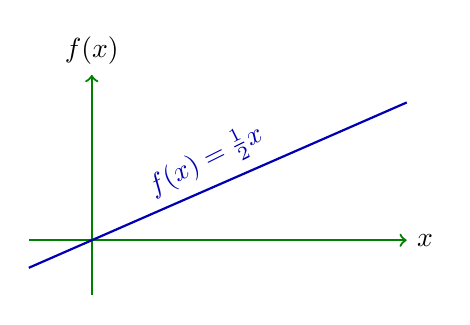
\begin{tikzpicture}
[
	xscale	= 0.8,	% to scale horizontally everything but the text
	yscale	= 0.7,	% to scale vertically everything but the text
]


\draw [->, color=black!50!green, thick] (-1,0) -- (5,0) node [right, color=black] {$x$};
\draw [->, color=black!50!green, thick] (0,-1) -- (0,3) node [above, color=black] {$f(x)$};
\draw [-, color=blue!70!black, thick] (-1,-0.5) -- (5,2.5) node [midway, above, sloped] {$f(x) = \frac{1}{2} x$};


\end{tikzpicture}
\end{center}
\end{figure}
 

	%
\end{frame}






\begin{frame}
	%
	\frametitle{Paths: how to set their terminations}
	%
	(example file: \url{./Sources/paths__caps_usage.tex} - requires \texttt{arrows} library)
	%
	

\begin{figure}[!htb]
\begin{center}
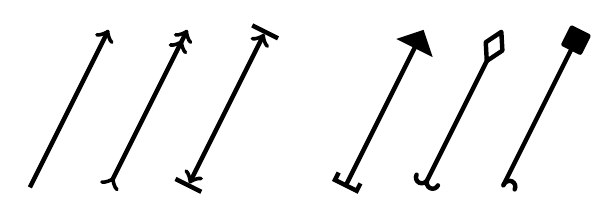
\begin{tikzpicture}
[
	xscale	= 1,	% to scale horizontally everything but the text
	yscale	= 1,	% to scale vertically everything but the text
]


\uncover<1->
{
	% not requiring ``arrows'' library
	\draw [ultra thick, ->]		(0,0) -- (1,2);
	\draw [ultra thick, >->>]	(1,0) -- (2,2);
	\draw [ultra thick, |<->|]	(2,0) -- (3,2);
}





\uncover<2->
{
	% requiring ``arrows'' library
	\draw [ultra thick, [-triangle 90]		(4,0) -- (5,2);
	\draw [ultra thick, hooks-open diamond]	(5,0) -- (6,2);
	\draw [ultra thick, left hook reversed-square]	(6,0) -- (7,2);
}


\end{tikzpicture}
\end{center}
\end{figure}




	%
\end{frame}






\begin{frame}
	%
	\frametitle{How to position text along a path}
	%
	(example file: \url{./Sources/paths__text_positioning.tex})
	%
	\begin{figure}[!htb]
\begin{center}
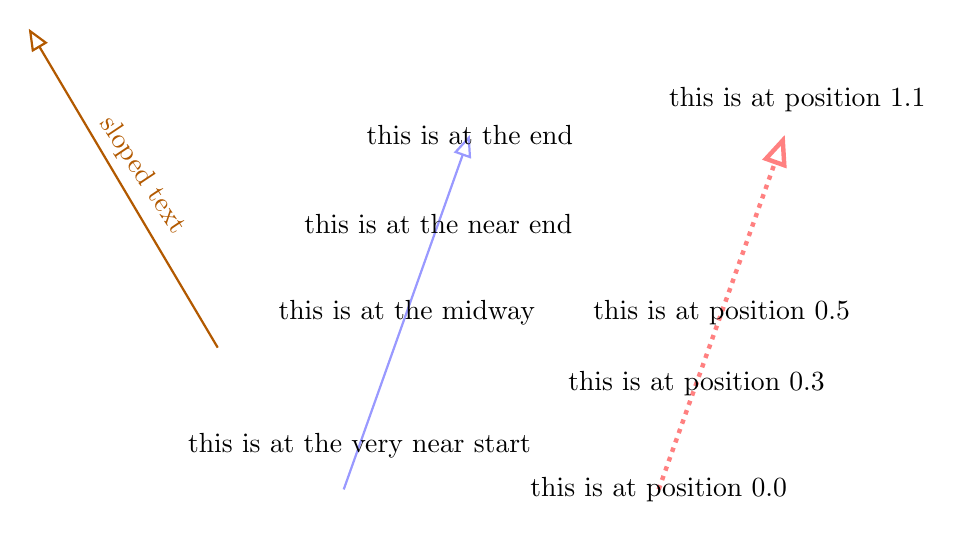
\begin{tikzpicture}
[
	xscale	= 0.8,	% to scale horizontally everything but the text
	yscale	= 0.9,	% to scale vertically everything but the text
]





\uncover<1->
{
	% intuitive positioning
	\draw
	[
		color	= blue!40,
		thick,
		-open triangle 45
	]
	(0,0) -- (2,5)
	node[black, at end]				{this is at the end}
	node[black, near end]			{this is at the near end}
	node[black, midway]				{this is at the midway}
	node[black, very near start]	{this is at the very near start};
}







\uncover<2->
{
	% numerical positioning
	\draw
	[
		color	= red!50,
		ultra thick,
		dotted,
		-open triangle 45
	]
	(5,0) -- (7,5)
	node[black, pos=0.0]			{this is at position 0.0}
	node[black, pos=0.3]			{this is at position 0.3}
	node[black, pos=0.5]			{this is at position 0.5}
	node[black, pos=1.1]			{this is at position 1.1};
}






\uncover<3->
{
	% sloping
	\draw
	[
		color	= black!30!orange,
		thick,
		-open triangle 45
	]
	(-2,2) -- (-5.0,6.5)
	node
	[				% here we define some properties of the node!
		midway,
		sloped,
		above,
		color = black!30!orange
	]
	{sloped text};
}




\end{tikzpicture}
\end{center}
\end{figure}

	%
\end{frame}

 



\begin{frame}
	%
	\frametitle{How to decorate paths}
	%
	(example file: \url{./Sources/paths__decorations.tex})
	%
	\begin{figure}[!htb]
\begin{center}
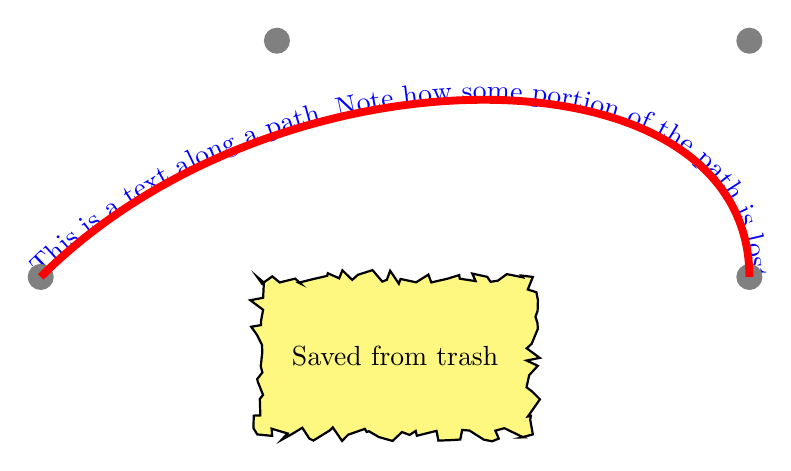
\begin{tikzpicture}
[
	xscale	= 1,	% to scale horizontally everything but the text
	yscale	= 1,	% to scale vertically everything but the text
]



\uncover<1->
{
	% text along a path
	\draw
	[
		decorate,
		decoration =
		{
			text along path,
			text color	= blue,
			text		= This is a text along a path. Note how some portion of the path is lost.
		}
	]
	(0,0) .. controls (3,3) and (9,3) .. (9,0);
}


\uncover<2-2>
{
	\node [circle, fill = gray, minimum size = 3mm] at (0,0) {};
	\node [circle, fill = gray, minimum size = 3mm] at (3,3) {};
	\node [circle, fill = gray, minimum size = 3mm] at (9,3) {};
	\node [circle, fill = gray, minimum size = 3mm] at (9,0) {};
	\draw
	[
		line width	= 0.1cm,
		color		= red,
	]
	(0,0) .. controls (3,3) and (9,3) .. (9,0);
}



\uncover<4->
{
	\node
	[
		draw,
		thick,
		minimum height	= 2cm,
		minimum width	= 3.5cm,
		fill			= yellow!50,
		inner xsep		= 0.3cm,
		inner ysep		= 0.3cm,
		decorate,
		decoration =
		{
			random steps,
			segment length	= 0.1cm,
			amplitude		= 0.09cm
		}
	]
	at (4.5,-1)
	{Saved from trash};
}



\end{tikzpicture}
\end{center}
\end{figure}


	%
\end{frame}


 
 
 

\section{Connection of nodes}
\label{sec:connection_of_nodes}




\begin{frame}
	%
	\frametitle{Straight connections using nodes' anchors}
	%
	(example file: \url{./Sources/connection_of_nodes__straight_connections.tex})
	%
	\input{connection_of_nodes__straight_connections}
	%
\end{frame}





\begin{frame}
	%
	\frametitle{Curved connections using nodes' anchors}
	%
	(example file: \url{./Sources/connection_of_nodes__curved_connections.tex})
	%
	
\begin{figure}[!htb]
\begin{center}
\begin{tikzpicture}
[
	xscale	= 1,	% to scale horizontally everything but the text
	yscale	= 1,	% to scale vertically everything but the text
]


\uncover<1->
{
	% nodes declaration
	\node (nGray)	[GenericNodeStyle, text=gray]	at	(-5, 0)	{gray};
	\node (nRed)	[GenericNodeStyle, text=red]	at	(1, 2)	{red};
	\node (nBlue)	[GenericNodeStyle, text=blue]	at	(1, -1)	{blue};
	\node (nYellow)	[GenericNodeStyle, text=yellow!80!black]	at	(4, 1.5)	{yellow};
}




\uncover<2->
{
	% first straight connection
	\draw
	[
		color	= black!40!white,
		ultra thick,
		->,
		out		= 90,
		in		= 180
	]
	(nGray) to (nRed); % NOTE: ``to'' AND NOT ``--''
}




\uncover<3->
{
	\draw
	[
		color	= blue,
		ultra thick,
		->,
		out		= 0,
		in		= 270
	]
	(nBlue.east) to (nYellow.240);
}




\end{tikzpicture}
\end{center}
\end{figure}


	%
\end{frame}






\begin{frame}
	%
	\frametitle{Straight connections using nodes' anchors - 2}
	%
	\small{(example file: \url{./Sources/connection_of_nodes__horizontal_vertical_connections.tex})}
	%
	\input{connection_of_nodes__horizontal_vertical_connections}
	%
\end{frame}





\section{Nets}
\label{sec:nets}


\begin{frame}
	%
	\frametitle{Example of sensor network}
	%
	(example file: \url{./Sources/nets__sensor_network.tex})
	%
	\begin{figure}[!htb]
\begin{center}
\begin{tikzpicture}
[
	xscale	= 1,	% to scale horizontally everything but the text
	yscale	= 1,	% to scale vertically everything but the text
]




\uncover<1->
{
	% bridges nodes
	\node	[BridgeNodeStyle]	(b1)	at	(0.8, 4.5)	{1};
	\node	[BridgeNodeStyle]	(b2)	at	(2.5, 0.8)	{2};
	\node	[BridgeNodeStyle]	(b3)	at	(4.3, 3.2)	{3};
	\node	[BridgeNodeStyle]	(b4)	at	(8.4, 4.8)	{4};
	%
	% normal nodes
	\node	[NormalNodeStyle]	(n5)	at	(2.0, 2.8)	{5};
	\node	[NormalNodeStyle]	(n6)	at	(3.1, 4.9)	{6};
	\node	[NormalNodeStyle]	(n7)	at	(4.1, 1.1)	{7};
	\node	[NormalNodeStyle]	(n8)	at	(6.1, 2.0)	{8};
	\node	[NormalNodeStyle]	(n9)	at	(5.0, 5.8)	{9};
	\node	[NormalNodeStyle]	(n10)	at	(6.0, 4.3)	{10};
	\node	[NormalNodeStyle]	(n11)	at	(7.7, 3.2)	{11};
}




\uncover<2->
{
	% connections
	\draw	[-, thick]	(b1) -- (n5);
	\draw	[-, thick]	(b1) -- (n6);
	%
	\draw	[-, thick]	(b2) -- (n7);
	%
	\draw	[-, thick]	(b3) -- (n6);
	\draw	[-, thick]	(b3) -- (n7);
	\draw	[-, thick]	(b3) -- (n8);
	%
	\draw	[-, thick]	(b4) -- (n9);
	\draw	[-, thick]	(b4) -- (n10);
	\draw	[-, thick]	(b4) -- (n11);
	%
	\draw	[-, thick]	(n7) -- (n8);
	\draw	[-, thick]	(n9) -- (n10);
	\draw	[-, thick]	(n10) -- (n11);
	%
	\draw	[triangle 60-triangle 60, thick, dotted]	(b3) -- (n10)
	node	[midway, above, sloped, font=\bfseries, text=red!70!black] {new};
}



\end{tikzpicture}
\end{center}
\end{figure}

	%
\end{frame}


\section{Block schemes}
\label{sec:block_schemes}



\begin{frame}
	%
	\frametitle{Block scheme example}
	%
	(example file: \url{./Sources/block_schemes__example.tex})
	%
	\begin{figure}[!htb]
\begin{center}
\begin{tikzpicture}
[
	xscale			= 1,	% to scale horizontally everything but the text
	yscale			= 1,	% to scale vertically everything but the text
]






\uncover<1->
{
	% blocks
	\node																	(nInput)		{$r$};
	\node [sSumBlockStyle,    right of=nInput,      node distance = 1.2cm]	(nSum)			{};
	\node [sNormalBlockStyle, right of=nSum,        node distance = 2.2cm]	(nController)	{controller};
	\node [sNormalBlockStyle, right of=nController, node distance = 3.4cm]	(nSystem)		{system};
	\node [                   above of=nSystem,     node distance = 1.5cm]	(nNoise)		{noise};
	\node [                   right of=nSystem,     node distance = 2.8cm]	(nOutput)		{$y$};
	%
	% auxiliary nodes
	\node 												(nAuxOne) at ($(nSystem)!0.7!(nOutput)$) {};
	\node [below of = nAuxOne, node distance = 1.3cm]	(nAuxTwo) {};
	%
	%
	% connections
	\draw [sArrowsStyle] (nInput)         -- (nSum)				node [very near end, above] {$+$};
	\draw [sArrowsStyle] (nSum)           -- (nController)		node [midway, above] {$e$};
	\draw [sArrowsStyle] (nController)    -- (nSystem)			node [above, midway] {$u$};
	\draw [sArrowsStyle] (nNoise)         -- (nSystem);
	\draw [sLinesStyle]  (nSystem)        -- (nAuxOne.center); % note the usage of ``.center''
	\draw [sArrowsStyle] (nAuxOne.center) -- (nOutput);
	\draw [sLinesStyle]  (nAuxOne.center) -- (nAuxTwo.center);
	\draw [sArrowsStyle] (nAuxTwo.center) -| (nSum)				node [near end, above right] {$-$};
}




\uncover<2-2> % only for understanding the construction of the figure
{
	\node [circle, fill = red, minimum size = 2mm] at (nAuxOne) {};
	\node [circle, fill = red, minimum size = 2mm] at (nAuxTwo) {};
}




\end{tikzpicture}
\end{center}
\end{figure}


	%
\end{frame}


\section{Warnings}


\begin{frame}
	%
	\frametitle{Warnings, i.e.\ what to \alert{do not} do}
	%
	\begin{itemize}
		%
		\item<2-> \alert{do not forget semicolons}; if compiler runs until $+\infty$ without responding then almost surely you forgot a semicolon
		%
		\item<3-> \alert{do not use numbers for the names of the nodes}; if you write \texttt{$\ldots$node (nMyNode1) [$\ldots$} you will get hundreds of errors!! Accepted syntax: \texttt{$\ldots$node (nMyNodeOne) [$\ldots$}
		%
		\item<4-> \alert{watch out in changing the order of the nodes / paths properties}: sometimes the compiler is not able to understand if things are written in a non-expected order
		%
		\item<5-> \alert{did you forgot to include the library?} Sometimes strange errors are due to the fact that you didn't include the opportune \Tikz library
		%
	\end{itemize}
	%
\end{frame}


\section{Mindmap}


\begin{frame}
\frametitle{Mindmap}


\begin{figure}
\begin{center}
\begin{tikzpicture}
[
%
transform canvas = {scale = 0.64},
mindmap,
text = black,
grow cyclic,
%
% ---------------------------------- styles
paths/.style =
{
	concept color	= blue!40,
	faded/.style	= {concept color = blue!40}
},
connections/.style =
{
	concept color	= orange!80,
	faded/.style	= {concept color = orange!40}
},
myNodes/.style =
{
	concept color	= yellow!80,
	faded/.style	= {concept color = yellow!40}
},
%
% ---------------------------------- general
every node/.style =
{
	concept,
	circular drop shadow,
	execute at begin node = \hskip0pt
},
%
% ---------------------------------- root
root concept/.append style =
{
	concept color	= black,
	fill			= white,
	line width		= 1ex,
	text			= black,
%	font			= \scshape
},
%
% ---------------------------------- first level
level 1/.append style =
{
	level distance	= 4.3cm,
	sibling angle	= -140,
%	font			= \scshape
},
%
% ---------------------------------- second level
level 2/.append style =
{
	level distance	= 3cm,
	sibling angle	= -60,
%	font			= \large
},
]



\node [root concept] {This Talk} % root
	child [myNodes]
	{
		node {Nodes}
		child
		{
			node {can be fully customized}
		}
		child
		{
			node {are labeled}
		}
		child
		{
			node {write inside using \LaTeX}
		}
	}
	child [paths]
	{
		node {Paths}
		child
		{
			node {connect everything}
		}
		child
		{
			node {can put labels on them}
		}
		child
		{
			node {used for decorations}
		}
	}
	child [connections]
	{
		node {Connections}
		child
		{
			node {straight}
		}
		child
		{
			node {curved}
		}
		child
		{
			node {horizontal / vertical}
		}
	}
;



\end{tikzpicture}
\end{center}
\end{figure}








\begin{tikzpicture}
[transform canvas = {scale = 0.3}]
\path
[
	xshift = -1.0cm,
	yshift = -10.5cm,
	draw = blue,
	decorate,
	decoration = 
	{
		text along path,
		text = {entirely written in |\color{red} \LaTeXe| ||using |\color{red} \texttt{Beamer}| ||and |\color{red}|Ti|||\color{red}\emph{k}| |||\color{red}|Z|| },
		text color = blue,
	}
]
(0,0) sin (1,1) cos (2,0) sin (3,-1) cos (4,0) sin (7,-1);
\end{tikzpicture}


\end{frame}




\begin{frame}
	%
	\begin{center}
	
\begin{tikzpicture}
		%
		\node
		[
			draw			= white!60!black,
			line width		= 0.2cm,
			minimum height	= 3cm,
			minimum width	= 5cm,
			inner xsep		= 0.3cm,
			inner ysep		= 0.3cm,
			decorate,
			decoration =
			{
				random steps,
				segment length	= 0.1cm,
				amplitude		= 0.09cm
			}
		]
		{\LARGE{\textbf{thank you}}};
		%
	\end{tikzpicture}
	\end{center}
	%
\end{frame}


%
\end{document}
%
%%%%%%%%%%%%%%%%%%%%%%%%%%%%%%%%%%%%%%%%%%%%%%%%%%%%%%%%%%%%%%%%%
